
\section{Disponibilidad de datos}
\label{sec:datos-apendice}

\section{Disponibilidad de códigos y reproducibilidad}
\label{sec:datos-reproducibilidad}

\section{Linaje de tablas GEIH}
\label{sec:apendice-linaje-geih}

    \begin{figure}[H]
    \centering
    \shorthandoff{>}
    \resizebox{\linewidth}{!}{%
    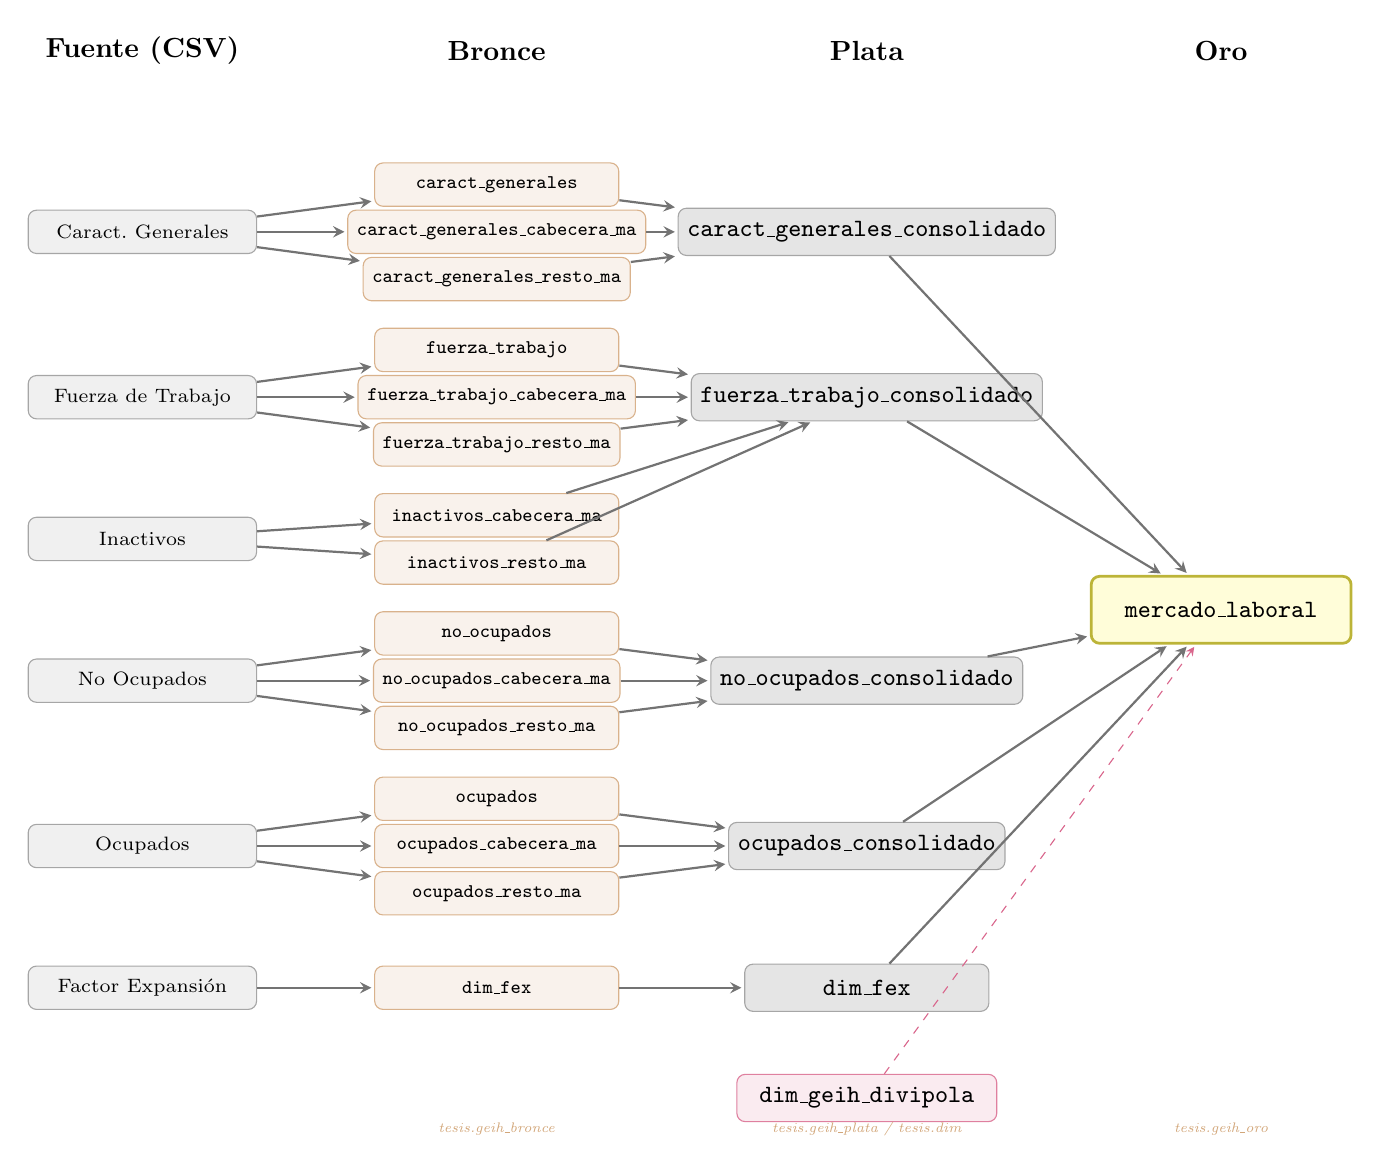
\begin{tikzpicture}[
        every node/.style={font=\small},
        fuente/.style={
            rectangle, rounded corners=3pt,
            draw=gray!70, fill=gray!12,
            minimum width=2.9cm, minimum height=0.55cm,
            text centered, align=center, font=\scriptsize
        },
        bronce/.style={
            rectangle, rounded corners=3pt,
            draw=brown!60, fill=brown!10,
            minimum width=3.1cm, minimum height=0.55cm,
            text centered, align=center, font=\scriptsize\ttfamily
        },
        plata/.style={
            rectangle, rounded corners=3pt,
            draw=gray!70, fill=gray!20,
            minimum width=3.1cm, minimum height=0.60cm,
            text centered, align=center, font=\small\ttfamily
        },
        dim/.style={
            rectangle, rounded corners=3pt,
            draw=purple!50, fill=purple!8,
            minimum width=3.3cm, minimum height=0.60cm,
            text centered, align=center, font=\small\ttfamily
        },
        oro/.style={
            rectangle, rounded corners=3pt,
            draw=yellow!70!black, fill=yellow!15, line width=1pt,
            minimum width=3.3cm, minimum height=0.85cm,
            text centered, align=center, font=\small\ttfamily\bfseries
        },
        arr/.style={->, >=stealth, thick, draw=black!55, shorten >=1pt},
        arrdim/.style={->, >=stealth, dashed, draw=purple!60, shorten >=1pt},
        hdr/.style={font=\normalsize\bfseries, text=black},
        note/.style={font=\tiny\itshape, text=brown!70}
    ]

    \def\xS{0}
    \def\xB{4.5}
    \def\xP{9.2}
    \def\xO{13.7}

    \node[hdr] at (\xS, 0.7) {Fuente (CSV)};
    \node[hdr] at (\xB, 0.7) {Bronce};
    \node[hdr] at (\xP, 0.7) {Plata};
    \node[hdr] at (\xO, 0.7) {Oro};

    % ── Características generales ──
    \node[fuente] (src_cg)  at (\xS,-1.6) {Caract.\ Generales};
    \node[bronce] (b_cg_n)  at (\xB,-1.0) {caract\_generales};
    \node[bronce] (b_cg_c)  at (\xB,-1.6) {caract\_generales\_cabecera\_ma};
    \node[bronce] (b_cg_r)  at (\xB,-2.2) {caract\_generales\_resto\_ma};
    \node[plata]  (p_cg)    at (\xP,-1.6) {caract\_generales\_consolidado};

    % ── Fuerza de trabajo ──
    \node[fuente] (src_ft)  at (\xS,-3.7) {Fuerza de Trabajo};
    \node[bronce] (b_ft_n)  at (\xB,-3.1) {fuerza\_trabajo};
    \node[bronce] (b_ft_c)  at (\xB,-3.7) {fuerza\_trabajo\_cabecera\_ma};
    \node[bronce] (b_ft_r)  at (\xB,-4.3) {fuerza\_trabajo\_resto\_ma};
    \node[plata]  (p_ft)    at (\xP,-3.7) {fuerza\_trabajo\_consolidado};

    % ── Inactivos (solo marco antiguo; alimenta fuerza\_trabajo) ──
    \node[fuente] (src_in)  at (\xS,-5.5) {Inactivos};
    \node[bronce] (b_in_c)  at (\xB,-5.2) {inactivos\_cabecera\_ma};
    \node[bronce] (b_in_r)  at (\xB,-5.8) {inactivos\_resto\_ma};

    % ── No ocupados ──
    \node[fuente] (src_no)  at (\xS,-7.3) {No Ocupados};
    \node[bronce] (b_no_n)  at (\xB,-6.7) {no\_ocupados};
    \node[bronce] (b_no_c)  at (\xB,-7.3) {no\_ocupados\_cabecera\_ma};
    \node[bronce] (b_no_r)  at (\xB,-7.9) {no\_ocupados\_resto\_ma};
    \node[plata]  (p_no)    at (\xP,-7.3) {no\_ocupados\_consolidado};

    % ── Ocupados ──
    \node[fuente] (src_oc)  at (\xS,-9.4) {Ocupados};
    \node[bronce] (b_oc_n)  at (\xB,-8.8) {ocupados};
    \node[bronce] (b_oc_c)  at (\xB,-9.4) {ocupados\_cabecera\_ma};
    \node[bronce] (b_oc_r)  at (\xB,-10.0) {ocupados\_resto\_ma};
    \node[plata]  (p_oc)    at (\xP,-9.4) {ocupados\_consolidado};

    % ── Factor de expansión ──
    \node[fuente] (src_fx)  at (\xS,-11.2) {Factor Expansión};
    \node[bronce] (b_fx)    at (\xB,-11.2) {dim\_fex};
    \node[plata]  (p_fx)    at (\xP,-11.2) {dim\_fex};

    % ── Oro + dimensión externa ──
    \node[oro] (o_ml)  at (\xO,-6.4)  {mercado\_laboral};
    \node[dim] (d_gdv) at (\xP,-12.6) {dim\_geih\_divipola};

    % ════ Fuente → Bronce ════
    \draw[arr] (src_cg) -- (b_cg_n);
    \draw[arr] (src_cg) -- (b_cg_c);
    \draw[arr] (src_cg) -- (b_cg_r);
    \draw[arr] (src_ft) -- (b_ft_n);
    \draw[arr] (src_ft) -- (b_ft_c);
    \draw[arr] (src_ft) -- (b_ft_r);
    \draw[arr] (src_in) -- (b_in_c);
    \draw[arr] (src_in) -- (b_in_r);
    \draw[arr] (src_no) -- (b_no_n);
    \draw[arr] (src_no) -- (b_no_c);
    \draw[arr] (src_no) -- (b_no_r);
    \draw[arr] (src_oc) -- (b_oc_n);
    \draw[arr] (src_oc) -- (b_oc_c);
    \draw[arr] (src_oc) -- (b_oc_r);
    \draw[arr] (src_fx) -- (b_fx);

    % ════ Bronce → Plata ════
    \draw[arr] (b_cg_n) -- (p_cg);
    \draw[arr] (b_cg_c) -- (p_cg);
    \draw[arr] (b_cg_r) -- (p_cg);
    \draw[arr] (b_ft_n) -- (p_ft);
    \draw[arr] (b_ft_c) -- (p_ft);
    \draw[arr] (b_ft_r) -- (p_ft);
    \draw[arr] (b_in_c) -- (p_ft);
    \draw[arr] (b_in_r) -- (p_ft);
    \draw[arr] (b_no_n) -- (p_no);
    \draw[arr] (b_no_c) -- (p_no);
    \draw[arr] (b_no_r) -- (p_no);
    \draw[arr] (b_oc_n) -- (p_oc);
    \draw[arr] (b_oc_c) -- (p_oc);
    \draw[arr] (b_oc_r) -- (p_oc);
    \draw[arr] (b_fx)   -- (p_fx);

    % ════ Plata → Oro ════
    \draw[arr] (p_cg) -- (o_ml);
    \draw[arr] (p_ft) -- (o_ml);
    \draw[arr] (p_no) -- (o_ml);
    \draw[arr] (p_oc) -- (o_ml);
    \draw[arr] (p_fx) -- (o_ml);
    \draw[arrdim] (d_gdv) -- (o_ml);

    \node[note] at (\xB, -13.0) {\textit{tesis.geih\_bronce}};
    \node[note] at (\xP, -13.0) {\textit{tesis.geih\_plata} / \textit{tesis.dim}};
    \node[note] at (\xO, -13.0) {\textit{tesis.geih\_oro}};

    \end{tikzpicture}%
    }% fin \resizebox
    \shorthandon{>}
    \caption{GEIH: linaje de tablas, de los archivos CSV de origen a la tabla de mercado laboral.}
    \label{fig:linaje_geih}
    \end{figure}

    \small
    \begin{longtable}{
        >{\raggedright\arraybackslash\ttfamily\footnotesize}p{6.0cm}
        >{\centering\arraybackslash}p{1.4cm}
        >{\raggedright\arraybackslash\ttfamily\footnotesize}p{5.6cm}
    }
    \caption{Tablas GEIH por capa en Unity Catalog y, para la capa bronce, el volumen del que se
    cargan. Las rutas son relativas a \texttt{/Volumes/tesis/geih\_bronce/}; las tablas plata y oro
    se derivan de otras tablas y no de un volumen.}
    \label{tab:tablas_geih_capa} \\
    \toprule
    \normalfont\textbf{Tabla} & \normalfont\textbf{Capa} & \normalfont\textbf{Volumen (ruta relativa)} \\
    \midrule
    \endfirsthead
    \multicolumn{3}{c}{\tablename\ \thetable{} (continuación)} \\
    \toprule
    \normalfont\textbf{Tabla} & \normalfont\textbf{Capa} & \normalfont\textbf{Volumen (ruta relativa)} \\
    \midrule
    \endhead
    \bottomrule
    \endfoot
    \bottomrule
    \endlastfoot
    caracteristicas\_\allowbreak generales & Bronce &
        caracteristicas\_\allowbreak generales/\allowbreak marco\_\allowbreak nuevo/\allowbreak *.csv \\
    caracteristicas\_\allowbreak generales\_\allowbreak area\_\allowbreak marco\_\allowbreak antiguo & Bronce &
        caracteristicas\_\allowbreak generales/\allowbreak marco\_\allowbreak antiguo/\allowbreak area/\allowbreak *.csv \\
    caracteristicas\_\allowbreak generales\_\allowbreak cabecera\_\allowbreak marco\_\allowbreak antiguo & Bronce &
        caracteristicas\_\allowbreak generales/\allowbreak marco\_\allowbreak antiguo/\allowbreak cabecera/\allowbreak *.csv \\
    caracteristicas\_\allowbreak generales\_\allowbreak resto\_\allowbreak marco\_\allowbreak antiguo & Bronce &
        caracteristicas\_\allowbreak generales/\allowbreak marco\_\allowbreak antiguo/\allowbreak resto/\allowbreak *.csv \\
    fuerza\_\allowbreak trabajo & Bronce &
        fuerza\_\allowbreak de\_\allowbreak trabajo/\allowbreak marco\_\allowbreak nuevo/\allowbreak *.csv \\
    fuerza\_\allowbreak trabajo\_\allowbreak area\_\allowbreak marco\_\allowbreak antiguo & Bronce &
        fuerza\_\allowbreak de\_\allowbreak trabajo/\allowbreak marco\_\allowbreak antiguo/\allowbreak area/\allowbreak *.csv \\
    fuerza\_\allowbreak trabajo\_\allowbreak cabecera\_\allowbreak marco\_\allowbreak antiguo & Bronce &
        fuerza\_\allowbreak de\_\allowbreak trabajo/\allowbreak marco\_\allowbreak antiguo/\allowbreak cabecera/\allowbreak *.csv \\
    fuerza\_\allowbreak trabajo\_\allowbreak resto\_\allowbreak marco\_\allowbreak antiguo & Bronce &
        fuerza\_\allowbreak de\_\allowbreak trabajo/\allowbreak marco\_\allowbreak antiguo/\allowbreak resto/\allowbreak *.csv \\
    inactivos\_\allowbreak area\_\allowbreak marco\_\allowbreak antiguo & Bronce &
        inactivos/\allowbreak marco\_\allowbreak antiguo/\allowbreak area/\allowbreak *.csv \\
    inactivos\_\allowbreak cabecera\_\allowbreak marco\_\allowbreak antiguo & Bronce &
        inactivos/\allowbreak marco\_\allowbreak antiguo/\allowbreak cabecera/\allowbreak *.csv \\
    inactivos\_\allowbreak resto\_\allowbreak marco\_\allowbreak antiguo & Bronce &
        inactivos/\allowbreak marco\_\allowbreak antiguo/\allowbreak resto/\allowbreak *.csv \\
    no\_\allowbreak ocupados & Bronce &
        no\_\allowbreak ocupados/\allowbreak marco\_\allowbreak nuevo/\allowbreak *.csv \\
    no\_\allowbreak ocupados\_\allowbreak area\_\allowbreak marco\_\allowbreak antiguo & Bronce &
        no\_\allowbreak ocupados/\allowbreak marco\_\allowbreak antiguo/\allowbreak area/\allowbreak *.csv \\
    no\_\allowbreak ocupados\_\allowbreak cabecera\_\allowbreak marco\_\allowbreak antiguo & Bronce &
        no\_\allowbreak ocupados/\allowbreak marco\_\allowbreak antiguo/\allowbreak cabecera/\allowbreak *.csv \\
    no\_\allowbreak ocupados\_\allowbreak resto\_\allowbreak marco\_\allowbreak antiguo & Bronce &
        no\_\allowbreak ocupados/\allowbreak marco\_\allowbreak antiguo/\allowbreak resto/\allowbreak *.csv \\
    ocupados & Bronce &
        ocupados/\allowbreak marco\_\allowbreak nuevo/\allowbreak *.csv \\
    ocupados\_\allowbreak area\_\allowbreak marco\_\allowbreak antiguo & Bronce &
        ocupados/\allowbreak marco\_\allowbreak antiguo/\allowbreak area/\allowbreak *.csv \\
    ocupados\_\allowbreak cabecera\_\allowbreak marco\_\allowbreak antiguo & Bronce &
        ocupados/\allowbreak marco\_\allowbreak antiguo/\allowbreak cabecera/\allowbreak *.csv \\
    ocupados\_\allowbreak resto\_\allowbreak marco\_\allowbreak antiguo & Bronce &
        ocupados/\allowbreak marco\_\allowbreak antiguo/\allowbreak resto/\allowbreak *.csv \\
    dim\_\allowbreak fex & Bronce & fex/\allowbreak *.csv \\
    \addlinespace
    caracteristicas\_\allowbreak generales\_\allowbreak consolidado & Plata & --- \\
    fuerza\_\allowbreak trabajo\_\allowbreak consolidado & Plata & --- \\
    no\_\allowbreak ocupados\_\allowbreak consolidado & Plata & --- \\
    ocupados\_\allowbreak consolidado & Plata & --- \\
    dim\_\allowbreak fex & Plata & --- \\
    \addlinespace
    mercado\_\allowbreak laboral & Oro & --- \\
    \end{longtable}

%--------------------------------------------------------------------------------------
%--------------------------------------------------------------------------------------
\section{Linaje de tablas TerriData}
\label{sec:apendice-linaje-terridata}

    \begin{figure}[H]
    \centering
    \shorthandoff{>}
    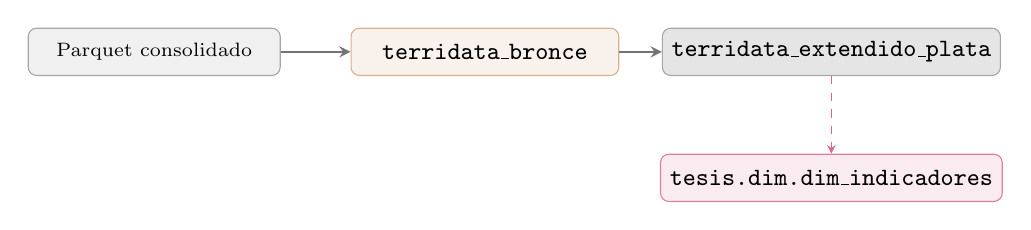
\begin{tikzpicture}[
        every node/.style={font=\small},
        fuente/.style={
            rectangle, rounded corners=3pt,
            draw=gray!70, fill=gray!12,
            minimum width=3.2cm, minimum height=0.60cm,
            text centered, align=center, font=\scriptsize
        },
        bronce/.style={
            rectangle, rounded corners=3pt,
            draw=brown!60, fill=brown!10,
            minimum width=3.4cm, minimum height=0.60cm,
            text centered, align=center, font=\small\ttfamily
        },
        plata/.style={
            rectangle, rounded corners=3pt,
            draw=gray!70, fill=gray!20,
            minimum width=3.6cm, minimum height=0.60cm,
            text centered, align=center, font=\small\ttfamily
        },
        externa/.style={
            rectangle, rounded corners=3pt,
            draw=purple!50, fill=purple!8,
            minimum width=3.8cm, minimum height=0.60cm,
            text centered, align=center, font=\small\ttfamily
        },
        arr/.style={->, >=stealth, thick, draw=black!55},
        arrdim/.style={->, >=stealth, dashed, draw=purple!60},
        hdr/.style={font=\normalsize\bfseries, text=black}
    ]

    \node[fuente]  (src)   at (0,-1)    {Parquet consolidado};
    \node[bronce]  (bronc) at (4.2,-1)  {terridata\_bronce};
    \node[plata]   (plata) at (8.6,-1)  {terridata\_extendido\_plata};
    \node[externa] (dimi)  at (8.6,-2.6) {tesis.dim.dim\_indicadores};

    \draw[arr]    (src)   -- (bronc);
    \draw[arr]    (bronc) -- (plata);
    \draw[arrdim] (plata) -- (dimi);

    \end{tikzpicture}
    \caption{TerriData: relación entre la fuente Parquet, la tabla bronce y la tabla plata
             pivoteada. La flecha punteada indica la tabla dimensional que \texttt{terridata\_extendido\_plata}
             genera en el esquema \texttt{tesis.dim}.}
    \label{fig:linaje_terridata}
    \end{figure}

    \begin{table}[H]
    \centering
    \small
    \begin{tabular}{>{\raggedright\arraybackslash\ttfamily}l >{\centering\arraybackslash}p{1.6cm}}
    \toprule
    \textbf{\normalfont Tabla} & \textbf{\normalfont Capa} \\
    \midrule
    terridata\_bronce & Bronce \\
    terridata\_extendido\_plata & Plata \\
    \bottomrule
    \end{tabular}
    \caption{Tablas del esquema \texttt{tesis.terridata}.}
    \label{tab:tablas_terridata}
    \end{table}

%--------------------------------------------------------------------------------------
\section{Linaje de tablas de dimensiones}
\label{sec:apendice-linaje-dim}

    \begin{figure}[H]
    \centering
    \shorthandoff{>}
    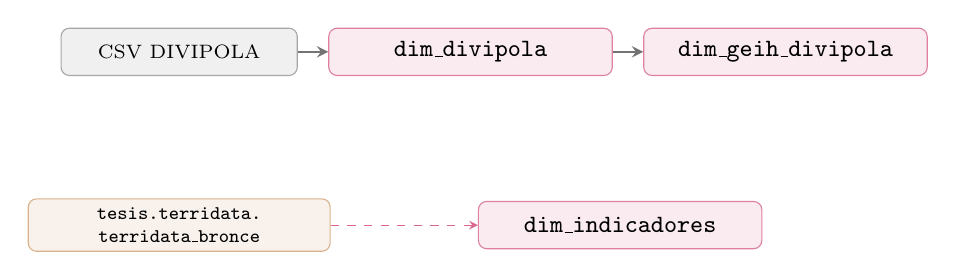
\begin{tikzpicture}[
        every node/.style={font=\small},
        fuente/.style={
            rectangle, rounded corners=3pt,
            draw=gray!70, fill=gray!12,
            minimum width=3.0cm, minimum height=0.60cm,
            text centered, align=center, font=\scriptsize
        },
        dim/.style={
            rectangle, rounded corners=3pt,
            draw=purple!50, fill=purple!8,
            minimum width=3.6cm, minimum height=0.60cm,
            text centered, align=center, font=\small\ttfamily
        },
        externa/.style={
            rectangle, rounded corners=3pt,
            draw=brown!60, fill=brown!10,
            text width=3.6cm, minimum height=0.60cm,
            text centered, align=center, font=\scriptsize\ttfamily
        },
        arr/.style={->, >=stealth, thick, draw=black!55},
        arrdim/.style={->, >=stealth, dashed, draw=purple!60}
    ]

    \node[fuente] (src)   at (0,-1)    {CSV DIVIPOLA};
    \node[dim]    (divi)  at (3.7,-1)  {dim\_divipola};
    \node[dim]    (gdivi) at (7.7,-1)  {dim\_geih\_divipola};

    \node[externa] (tbron) at (0,-3.2)   {tesis.terridata.\\terridata\_bronce};
    \node[dim]     (dind)  at (5.6,-3.2) {dim\_indicadores};

    \draw[arr]    (src)  -- (divi);
    \draw[arr]    (divi) -- (gdivi);
    \draw[arrdim] (tbron) -- (dind);

    \end{tikzpicture}
    \caption{Dimensiones: \texttt{dim\_divipola} se construye desde el catálogo territorial en CSV y
             \texttt{dim\_geih\_divipola} filtra sus 32 ciudades GEIH. \texttt{dim\_indicadores} es
             generada externamente por la capa plata de TerriData (flecha punteada), no por un
             notebook propio de este esquema.}
    \label{fig:linaje_dim}
    \end{figure}

    \begin{table}[H]
    \centering
    \small
    \begin{tabular}{>{\raggedright\arraybackslash\ttfamily}l}
    \toprule
    \textbf{\normalfont Tabla} \\
    \midrule
    dim\_divipola \\
    dim\_geih\_divipola \\
    dim\_indicadores \\
    \bottomrule
    \end{tabular}
    \caption{Tablas del esquema \texttt{tesis.dim}.}
    \label{tab:tablas_dim}
    \end{table}

%--------------------------------------------------------------------------------------
\section{Linaje de tablas de preprocesamiento}
\label{sec:apendice-linaje-preprocesamiento}

    \begin{figure}[H]
    \centering
    \shorthandoff{>}
    \resizebox{\linewidth}{!}{%
    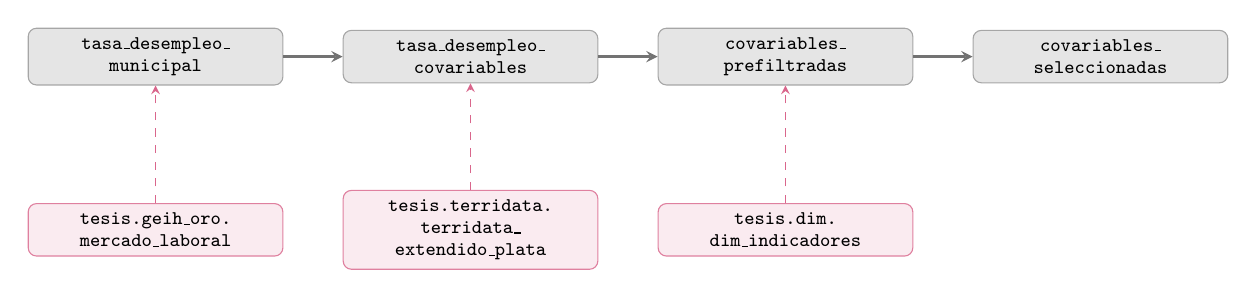
\begin{tikzpicture}[
        every node/.style={font=\small},
        plata/.style={
            rectangle, rounded corners=3pt,
            draw=gray!70, fill=gray!20,
            text width=3.0cm, minimum height=0.60cm,
            text centered, align=center, font=\scriptsize\ttfamily
        },
        externa/.style={
            rectangle, rounded corners=3pt,
            draw=purple!50, fill=purple!8,
            text width=3.0cm, minimum height=0.60cm,
            text centered, align=center, font=\scriptsize\ttfamily
        },
        arr/.style={->, >=stealth, thick, draw=black!55},
        arrdim/.style={->, >=stealth, dashed, draw=purple!60}
    ]

    \node[plata]   (tdm)  at (0,-1)   {tasa\_\allowbreak desempleo\_\allowbreak municipal};
    \node[plata]   (tdc)  at (4.0,-1) {tasa\_\allowbreak desempleo\_\allowbreak covariables};
    \node[plata]   (cpf)  at (8.0,-1) {covariables\_\allowbreak prefiltradas};
    \node[plata]   (cs)   at (12.0,-1) {covariables\_\allowbreak seleccionadas};

    \node[externa] (ml)   at (0,-3.2)   {tesis.geih\_oro.\\mercado\_\allowbreak laboral};
    \node[externa] (tdp)  at (4.0,-3.2) {tesis.terridata.\\terridata\_\allowbreak extendido\_\allowbreak plata};
    \node[externa] (dind) at (8.0,-3.2) {tesis.dim.\\dim\_\allowbreak indicadores};

    \draw[arr]    (tdm) -- (tdc);
    \draw[arr]    (tdc) -- (cpf);
    \draw[arr]    (cpf) -- (cs);
    \draw[arrdim] (ml)   -- (tdm);
    \draw[arrdim] (tdp)  -- (tdc);
    \draw[arrdim] (dind) -- (cpf);

    \end{tikzpicture}%
    }% fin \resizebox
    \caption{Preprocesamiento: de la tasa de desempleo municipal (estimador de Hájek sobre
             \texttt{mercado\_laboral}) a las covariables seleccionadas por el análisis
             exploratorio. Las flechas punteadas señalan tablas externas al esquema.}
    \label{fig:linaje_preprocesamiento}
    \end{figure}

    \begin{table}[H]
    \centering
    \small
    \begin{tabular}{>{\raggedright\arraybackslash\ttfamily}l}
    \toprule
    \textbf{\normalfont Tabla} \\
    \midrule
    tasa\_desempleo\_municipal \\
    tasa\_desempleo\_covariables \\
    covariables\_prefiltradas \\
    covariables\_seleccionadas \\
    \midrule
    covariables\_prefiltradas\_rev \\
    cascada\_prefiltrado\_rev \\
    sensibilidad\_variabilidad\_rev \\
    covariables\_candidatas\_rev \\
    descriptivo\_univariado\_rev \\
    descriptivo\_bivariado\_rev \\
    diagnosticos\_covariables\_rev \\
    robustez\_covariables\_rev \\
    redundancia\_covariables\_rev \\
    busqueda\_aic\_rev \\
    verificacion\_seleccion\_rev \\
    trazabilidad\_covariables\_rev \\
    covariables\_seleccionadas\_rev \\
    municipios\_sin\_encuesta\_rev \\
    \bottomrule
    \end{tabular}
    \caption{Tablas del esquema \texttt{tesis.preprocesamiento}. Bajo la línea intermedia, las tablas con sufijo \texttt{\_rev} que produce el procedimiento revisado; las anteriores se conservan sin modificación para permitir la comparación entre ambos procedimientos.}
    \label{tab:tablas_preprocesamiento}
    \end{table}

%--------------------------------------------------------------------------------------
\section{Linaje de tablas del modelo}
\label{sec:apendice-linaje-modelo}

    \begin{figure}[H]
    \centering
    \shorthandoff{>}
    \resizebox{\linewidth}{!}{%
    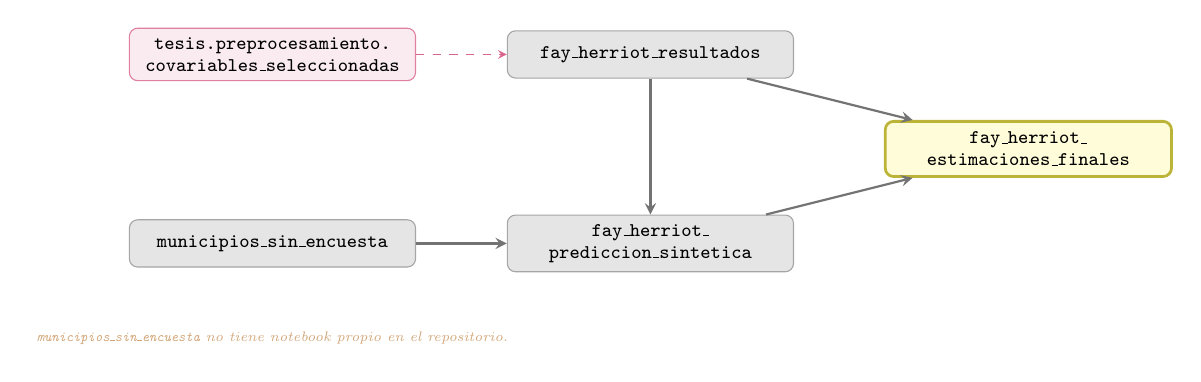
\begin{tikzpicture}[
        every node/.style={font=\small},
        plata/.style={
            rectangle, rounded corners=3pt,
            draw=gray!70, fill=gray!20,
            text width=3.4cm, minimum height=0.60cm,
            text centered, align=center, font=\scriptsize\ttfamily
        },
        oro/.style={
            rectangle, rounded corners=3pt,
            draw=yellow!70!black, fill=yellow!15, line width=1pt,
            text width=3.4cm, minimum height=0.70cm,
            text centered, align=center, font=\scriptsize\ttfamily\bfseries
        },
        externa/.style={
            rectangle, rounded corners=3pt,
            draw=purple!50, fill=purple!8,
            text width=3.4cm, minimum height=0.60cm,
            text centered, align=center, font=\scriptsize\ttfamily
        },
        arr/.style={->, >=stealth, thick, draw=black!55},
        arrdim/.style={->, >=stealth, dashed, draw=purple!60},
        note/.style={font=\tiny\itshape, text=brown!70}
    ]

    \node[externa] (cs)  at (0,-1)     {tesis.preprocesamiento.\\covariables\_\allowbreak seleccionadas};
    \node[plata]   (fhr) at (4.8,-1)   {fay\_\allowbreak herriot\_\allowbreak resultados};

    \node[plata]   (mse) at (0,-3.4)   {municipios\_\allowbreak sin\_\allowbreak encuesta};
    \node[plata]   (fhp) at (4.8,-3.4) {fay\_\allowbreak herriot\_\allowbreak prediccion\_\allowbreak sintetica};

    \node[oro]     (fhe) at (9.6,-2.2) {fay\_\allowbreak herriot\_\allowbreak estimaciones\_\allowbreak finales};

    \draw[arrdim] (cs)  -- (fhr);
    \draw[arr]    (mse) -- (fhp);
    \draw[arr]    (fhr) -- (fhp);
    \draw[arr]    (fhr) -- (fhe);
    \draw[arr]    (fhp) -- (fhe);

    \node[note] at (0,-4.6) {\texttt{municipios\_sin\_encuesta} no tiene notebook propio en el repositorio.};

    \end{tikzpicture}%
    }% fin \resizebox
    \caption{Modelo: del ajuste del Fay-Herriot ganador (\texttt{fay\_herriot\_resultados}) y la
             predicción sintética para dominios sin encuesta a la tabla final consolidada. La
             flecha punteada señala la tabla externa de entrada. Se excluyen del análisis
             \texttt{cargas\_pca\_ganadoras\_opcion\_a} y
             \texttt{cargas\_pca\_ganadoras\_opcion\_b\_hibrida}.}
    \label{fig:linaje_modelo}
    \end{figure}

    \begin{table}[H]
    \centering
    \small
    \begin{tabular}{>{\raggedright\arraybackslash\ttfamily}l}
    \toprule
    \textbf{\normalfont Tabla} \\
    \midrule
    municipios\_sin\_encuesta \\
    fay\_herriot\_resultados \\
    fay\_herriot\_prediccion\_sintetica \\
    fay\_herriot\_estimaciones\_finales \\
    \midrule
    fh\_diagnosticos\_variantes\_rev \\
    fh\_seleccion\_modelo\_rev \\
    fh\_coeficientes\_rev \\
    fay\_herriot\_resultados\_rev \\
    fay\_herriot\_prediccion\_sintetica\_rev \\
    fay\_herriot\_estimaciones\_finales\_rev \\
    \bottomrule
    \end{tabular}
    \caption{Tablas del esquema \texttt{tesis.modelo}. Bajo la línea intermedia, las tablas con sufijo \texttt{\_rev} que produce el procedimiento revisado; las anteriores se conservan sin modificación para permitir la comparación entre ambos procedimientos.}
    \label{tab:tablas_modelo}
    \end{table}


%--------------------------------------------------------------------------------------
\section{Estimaciones sintéticas por municipio}
\label{sec:apendice-sinteticas}

    La Tabla~\ref{tab:prediccion_sintetica} reporta, municipio por municipio, las estimaciones sintéticas del modelo elegido M2 para los 82 municipios del Cauca y del Valle del Cauca sin cobertura muestral de la GEIH, obtenidas según la Sección~\ref{sec:met_sintetico}. Su resumen por departamento se presenta en la Tabla~\ref{tab:resumen_sintetico}: ninguna estimación es confiable, 40 son aceptables y 42 no confiables, y 76 llevan la marca de extrapolación.

\small
\begin{longtable}{p{3.4cm} r r r l c}
\caption{Estimación sintética de la tasa de desempleo para los 82 municipios sin cobertura
muestral de la GEIH, obtenida con el modelo M2. Estimación: $\mathbf{x}_d^\top\hat{\boldsymbol{\beta}}$
en porcentaje; RMSE: raíz del error cuadrático medio de la Ecuación~\ref{eq:var_sintetica}, en
puntos porcentuales; CV: coeficiente de variación en porcentaje. La confiabilidad aplica los
umbrales de la Tabla~\ref{tab:criterios_decision}: confiable por debajo del 5\%, aceptable entre el
5\% y el 20\% y no confiable a partir del 20\%. Extrapola: marca de la
Ecuación~\ref{eq:extrapolacion}. Los municipios se agrupan por departamento.}
\label{tab:prediccion_sintetica} \\
\toprule
\textbf{Municipio} & \textbf{Estimación} & \textbf{RMSE} & \textbf{CV} & \textbf{Confiabilidad} & \textbf{Extrapola} \\
\midrule
\endfirsthead
\multicolumn{6}{c}{\tablename\ \thetable{} (continuación)} \\
\toprule
\textbf{Municipio} & \textbf{Estimación} & \textbf{RMSE} & \textbf{CV} & \textbf{Confiabilidad} & \textbf{Extrapola} \\
\midrule
\endhead
\bottomrule
\endfoot
\bottomrule
\endlastfoot
\multicolumn{6}{l}{\textbf{Cauca}} \\
Almaguer & 21.04 & 3.46 & 16.43 & Aceptable & Sí \\
Argelia & 18.02 & 2.84 & 15.78 & Aceptable & Sí \\
Balboa & 23.50 & 4.73 & 20.14 & No confiable & Sí \\
Bolívar & 18.79 & 3.08 & 16.41 & Aceptable & Sí \\
Buenos Aires & 27.59 & 6.58 & 23.86 & No confiable & Sí \\
Cajibío & 23.26 & 4.26 & 18.33 & Aceptable & Sí \\
Caldono & 23.29 & 4.85 & 20.84 & No confiable & Sí \\
Caloto & 14.88 & 2.57 & 17.24 & Aceptable & Sí \\
Corinto & 18.97 & 4.31 & 22.72 & No confiable & Sí \\
El Tambo & 29.87 & 8.37 & 28.03 & No confiable & Sí \\
Florencia & 18.55 & 4.33 & 23.31 & No confiable & Sí \\
Guachené & 24.35 & 6.01 & 24.67 & No confiable & Sí \\
Guapi & 20.34 & 3.84 & 18.87 & Aceptable & Sí \\
Inzá & 21.10 & 4.25 & 20.12 & No confiable & Sí \\
Jambaló & 17.63 & 2.76 & 15.64 & Aceptable & Sí \\
La Sierra & 23.64 & 5.07 & 21.43 & No confiable & Sí \\
La Vega & 24.31 & 4.25 & 17.48 & Aceptable & Sí \\
López & 31.54 & 6.44 & 20.42 & No confiable & Sí \\
Mercaderes & 21.42 & 3.56 & 16.63 & Aceptable & Sí \\
Miranda & 14.31 & 2.37 & 16.57 & Aceptable & No \\
Morales & 24.08 & 4.77 & 19.80 & Aceptable & Sí \\
Padilla & 25.12 & 6.84 & 27.22 & No confiable & Sí \\
Paéz & 25.89 & 4.79 & 18.50 & Aceptable & Sí \\
Patía & 18.68 & 3.19 & 17.09 & Aceptable & Sí \\
Piamonte & 36.01 & 10.66 & 29.60 & No confiable & Sí \\
Piendamó & 18.84 & 3.68 & 19.53 & Aceptable & Sí \\
Puerto Tejada & 13.77 & 2.61 & 18.96 & Aceptable & Sí \\
Puracé & 23.72 & 4.56 & 19.23 & Aceptable & Sí \\
Rosas & 20.54 & 3.83 & 18.67 & Aceptable & Sí \\
San Sebastián & 21.54 & 3.60 & 16.70 & Aceptable & Sí \\
Santa Rosa & 21.01 & 3.50 & 16.65 & Aceptable & Sí \\
Santander de Quilichao & 17.54 & 3.21 & 18.28 & Aceptable & Sí \\
Silvia & 18.27 & 3.00 & 16.41 & Aceptable & Sí \\
Sotará & 22.58 & 4.31 & 19.08 & Aceptable & Sí \\
Suárez & 23.72 & 4.29 & 18.07 & Aceptable & Sí \\
Sucre & 27.60 & 5.39 & 19.54 & Aceptable & Sí \\
Timbío & 20.83 & 4.23 & 20.31 & No confiable & Sí \\
Timbiquí & 27.82 & 5.13 & 18.43 & Aceptable & Sí \\
Toribío & 17.93 & 2.79 & 15.55 & Aceptable & Sí \\
Totoró & 23.83 & 4.19 & 17.57 & Aceptable & Sí \\
Villa Rica & 19.87 & 3.69 & 18.59 & Aceptable & Sí \\
\midrule
\multicolumn{6}{l}{\textbf{Valle del Cauca}} \\
Alcalá & 25.83 & 6.16 & 23.84 & No confiable & Sí \\
Andalucía & 24.17 & 5.79 & 23.94 & No confiable & Sí \\
Ansermanuevo & 27.44 & 7.33 & 26.73 & No confiable & Sí \\
Argelia & 29.36 & 8.49 & 28.93 & No confiable & Sí \\
Bolívar & 27.38 & 7.62 & 27.85 & No confiable & Sí \\
Buenaventura & 16.48 & 2.85 & 17.27 & Aceptable & Sí \\
Bugalagrande & 17.55 & 2.98 & 17.00 & Aceptable & Sí \\
Caicedonia & 27.82 & 7.73 & 27.79 & No confiable & Sí \\
Calima & 13.85 & 2.23 & 16.13 & Aceptable & No \\
Candelaria & 17.99 & 3.53 & 19.63 & Aceptable & Sí \\
Cartago & 14.21 & 2.40 & 16.86 & Aceptable & No \\
Dagua & 26.44 & 6.56 & 24.80 & No confiable & Sí \\
El Águila & 27.56 & 7.32 & 26.55 & No confiable & Sí \\
El Cairo & 30.30 & 8.76 & 28.92 & No confiable & Sí \\
El Cerrito & 17.47 & 3.67 & 21.00 & No confiable & Sí \\
El Dovio & 26.64 & 6.72 & 25.22 & No confiable & Sí \\
Florida & 17.77 & 3.68 & 20.70 & No confiable & Sí \\
Ginebra & 17.68 & 4.80 & 27.18 & No confiable & Sí \\
Guacarí & 24.21 & 6.23 & 25.73 & No confiable & Sí \\
Guadalajara de Buga & 13.42 & 2.34 & 17.46 & Aceptable & No \\
Jamundí & 16.74 & 3.04 & 18.15 & Aceptable & Sí \\
La Cumbre & 24.28 & 6.36 & 26.21 & No confiable & Sí \\
La Unión & 20.72 & 4.88 & 23.54 & No confiable & Sí \\
La Victoria & 20.50 & 5.75 & 28.02 & No confiable & Sí \\
Obando & 32.76 & 9.45 & 28.85 & No confiable & Sí \\
Palmira & 15.04 & 2.71 & 18.00 & Aceptable & Sí \\
Pradera & 19.62 & 3.87 & 19.74 & Aceptable & Sí \\
Restrepo & 26.40 & 9.07 & 34.35 & No confiable & Sí \\
Riofrío & 25.32 & 7.04 & 27.80 & No confiable & Sí \\
Roldanillo & 18.54 & 4.53 & 24.44 & No confiable & Sí \\
San Pedro & 32.38 & 10.84 & 33.48 & No confiable & Sí \\
Sevilla & 24.41 & 6.20 & 25.40 & No confiable & Sí \\
Toro & 23.76 & 5.56 & 23.42 & No confiable & Sí \\
Trujillo & 26.84 & 7.04 & 26.25 & No confiable & Sí \\
Tuluá & 13.80 & 2.37 & 17.17 & Aceptable & No \\
Ulloa & 26.91 & 6.85 & 25.44 & No confiable & Sí \\
Versalles & 23.34 & 5.02 & 21.53 & No confiable & Sí \\
Vijes & 27.97 & 8.30 & 29.66 & No confiable & Sí \\
Yotoco & 23.68 & 6.03 & 25.46 & No confiable & Sí \\
Yumbo & 10.60 & 2.10 & 19.78 & Aceptable & No \\
Zarzal & 15.46 & 2.61 & 16.91 & Aceptable & Sí \\
\end{longtable}
\normalsize

%--------------------------------------------------------------------------------------
\section{Variantes del modelo Fay-Herriot}
\label{sec:apendice-variantes}

    Esta sección reúne las cifras de las cinco variantes de la Tabla~\ref{tab:variantes_modelo}, de las que el capítulo de resultados presenta solo el modelo elegido M2. Todas se ajustaron con el procedimiento de la Sección~\ref{subsec:met_estimacion} y se evaluaron con los diagnósticos de las Secciones~\ref{subsec:met_validacion} y~\ref{subsec:met_robustez_fh}.

    La Tabla~\ref{tab:coef_variantes} reporta los coeficientes de cada variante. En ninguna todas las covariables son significativas al 5\%, condición que se discute en la Sección~\ref{subsec:res_criterio_seleccion}. Cada covariable conserva su signo en todas las variantes que la incluyen. La varianza de los efectos aleatorios va de 3.960 en M2 a 4.595 en M4.

    \begin{table}[!htbp]
    \centering
    \footnotesize
    \caption{Coeficientes de las cinco variantes del modelo de Fay-Herriot, estimados por mínimos
             cuadrados generalizados, con el error estándar entre paréntesis y el valor $p$ de la
             Ecuación~\ref{eq:cov_beta} debajo. Media: cobertura neta en educación media;
             Secundaria: cobertura neta en educación secundaria; VA primario: participación de
             las actividades primarias en el valor agregado; IPM: índice de pobreza
             multidimensional. Las celdas vacías corresponden a covariables que no forman parte
             de la variante. M2 es el modelo elegido.}
    \label{tab:coef_variantes}
    \renewcommand{\arraystretch}{1.15}
    \setlength{\tabcolsep}{4pt}
    \begin{tabular}{l r r r r r}
    \toprule
    \textbf{Parámetro} & \textbf{M1} & \textbf{M2} & \textbf{M3} & \textbf{M4} & \textbf{M5} \\
    \midrule
    Intercepto  & 23.475 & 23.332 & 18.251 & 25.394 & 25.516 \\
                & (7.976) & (7.681) & (6.676) & (8.136) & (6.810) \\
                & $p=0.003$ & $p=0.002$ & $p=0.006$ & $p=0.002$ & $p<0.001$ \\[3pt]
    Media       & $-$0.023 &  & $-$0.162 & $-$0.083 & $-$0.066 \\
                & (0.164) &  & (0.113) & (0.164) & (0.139) \\
                & $p=0.888$ &  & $p=0.152$ & $p=0.612$ & $p=0.637$ \\[3pt]
    Secundaria  & $-$0.146 & $-$0.159 &  & $-$0.126 & $-$0.137 \\
                & (0.125) & (0.083) &  & (0.129) & (0.121) \\
                & $p=0.244$ & $p=0.056$ &  & $p=0.327$ & $p=0.259$ \\[3pt]
    VA primario & 0.292 & 0.299 & 0.267 &  & 0.302 \\
                & (0.196) & (0.185) & (0.197) &  & (0.191) \\
                & $p=0.137$ & $p=0.106$ & $p=0.175$ &  & $p=0.114$ \\[3pt]
    IPM         & 0.037 & 0.041 & 0.025 & 0.048 &  \\
                & (0.070) & (0.059) & (0.070) & (0.072) &  \\
                & $p=0.601$ & $p=0.486$ & $p=0.719$ & $p=0.510$ &  \\
    \midrule
    $\hat{\sigma}_u^2$ & 4.232 & 3.960 & 4.346 & 4.595 & 4.006 \\
    AIC                & 110.348 & 108.376 & 110.026 & 111.013 & 108.663 \\
    \bottomrule
    \end{tabular}
    \end{table}
    \FloatBarrier

    La Tabla~\ref{tab:diagnosticos_variantes} reúne los diagnósticos de las cinco variantes. Todas presentan residuos con media compatible con cero, desviación estándar entre 0.902 y 0.928 y normalidad no rechazada por la prueba de Shapiro-Wilk. En todas el error cuadrático medio del EBLUP es inferior a la varianza directa en los 23 dominios, con razón media entre 1.155 y 1.180. La correlación del efecto suavizador va de 0.723 en M1 a 0.792 en M4, y el $R^2$ del predictor sintético de 0.331 en M4 a 0.403 en M1. M4 es la única variante con un dominio por encima del umbral de Cook, Valledupar, con 0.181.

    \begin{table}[!htbp]
    \centering
    \small
    \caption{Diagnósticos de las cinco variantes. $R^2$: coeficiente de determinación del predictor
             sintético; Media y DE: media y desviación estándar de los residuos estandarizados de
             la Ecuación~\ref{eq:residuos}; SW: valor $p$ de Shapiro-Wilk; $\bar{\gamma}$: factor
             de contracción promedio; $\bar{R}_d$: razón media de la Ecuación~\ref{eq:ratio_mse},
             con $R_d > 1$ en los 23 dominios de todas las variantes y valor $p$ de Wilcoxon
             inferior a 0.001; $r_{\text{suav}}$: correlación del efecto suavizador, con valor $p$
             inferior a 0.001; Cook: distancia de Cook máxima de la Ecuación~\ref{eq:cook_gls},
             con umbral 0.174.}
    \label{tab:diagnosticos_variantes}
    \renewcommand{\arraystretch}{1.25}
    \begin{tabular}{l r r r r r r r r}
    \toprule
    \textbf{Modelo} & \textbf{$R^2$} & \textbf{Media} & \textbf{DE} & \textbf{SW} &
    \textbf{$\bar{\gamma}$} & \textbf{$\bar{R}_d$} & \textbf{$r_{\text{suav}}$} & \textbf{Cook} \\
    \midrule
    M1 & 0.403 & 0.020 & 0.902 & 0.508 & 0.788 & 1.155 & 0.723 & 0.158 \\
    M2 & 0.402 & 0.021 & 0.926 & 0.577 & 0.777 & 1.178 & 0.724 & 0.122 \\
    M3 & 0.360 & 0.019 & 0.925 & 0.484 & 0.792 & 1.163 & 0.756 & 0.139 \\
    M4 & 0.331 & 0.022 & 0.925 & 0.358 & 0.801 & 1.156 & 0.792 & 0.181 \\
    M5 & 0.390 & 0.022 & 0.928 & 0.498 & 0.779 & 1.180 & 0.746 & 0.141 \\
    \bottomrule
    \end{tabular}
    \end{table}
    \FloatBarrier

    Las Figuras~\ref{fig:ap_suavizador_variantes} y~\ref{fig:ap_histograma_variantes} presentan el efecto suavizador y el histograma de residuos de las cuatro variantes no elegidas, con la misma lectura que las Figuras~\ref{fig:fh_suavizador} y~\ref{fig:fh_histograma} del modelo elegido.

    \begin{figure}[!htbp]
    \centering
    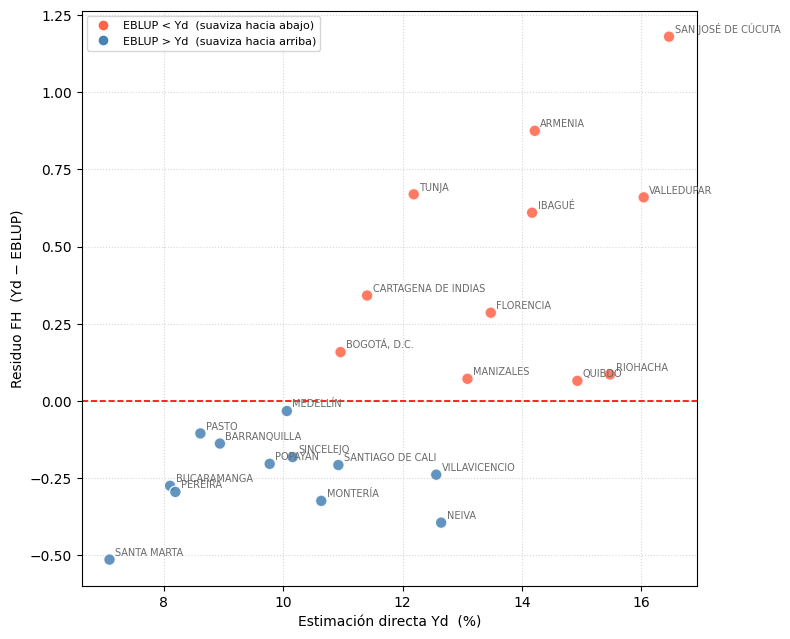
\includegraphics[width=0.48\textwidth]{img/fh_var1_suavizador.png}
    \hfill
    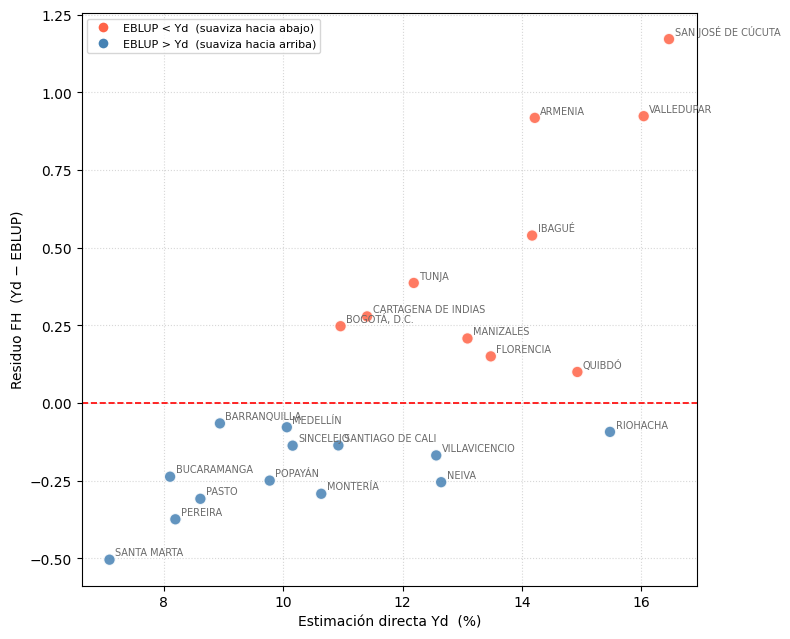
\includegraphics[width=0.48\textwidth]{img/fh_var3_suavizador.png}
    \\[6pt]
    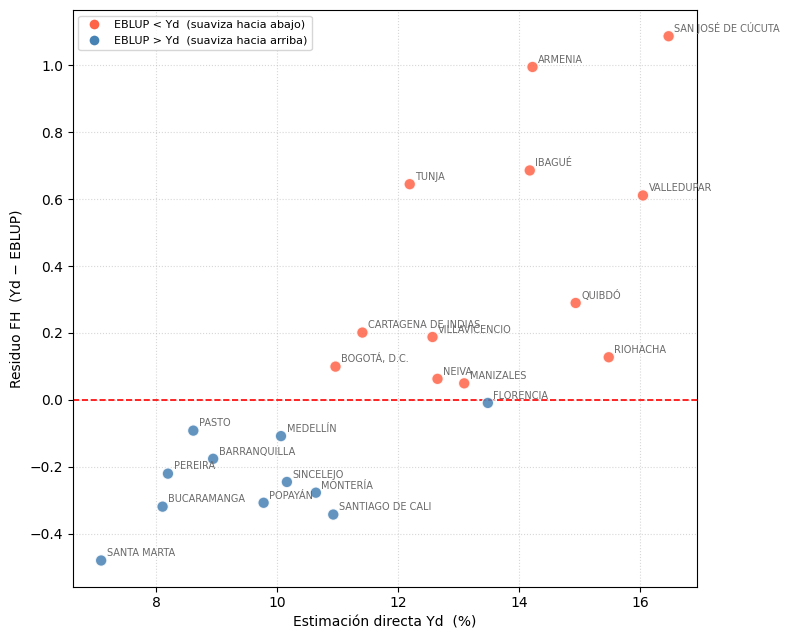
\includegraphics[width=0.48\textwidth]{img/fh_var4_suavizador.png}
    \hfill
    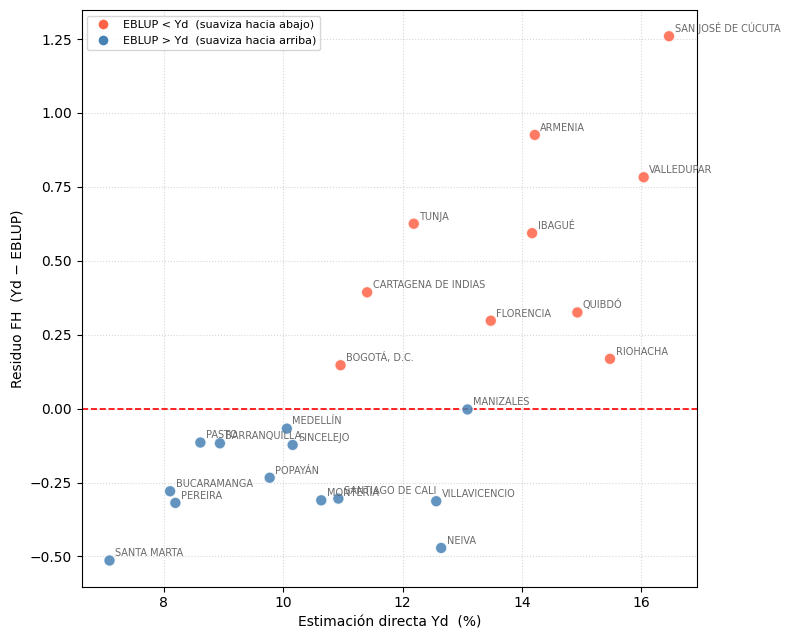
\includegraphics[width=0.48\textwidth]{img/fh_var5_suavizador.png}
    \caption{Efecto suavizador de las variantes no elegidas: arriba a la izquierda M1, arriba a la
             derecha M3, abajo a la izquierda M4 y abajo a la derecha M5. Cada panel enfrenta la
             estimación directa $\hat{\theta}_d$ con la corrección
             $\hat{\theta}_d - \hat{\theta}_d^{\text{EBLUP}}$ de la
             Ecuación~\ref{eq:correccion_eblup}; los puntos rojos son dominios cuya estimación el
             EBLUP modera y los azules dominios cuya estimación eleva.}
    \label{fig:ap_suavizador_variantes}
    \end{figure}
    \FloatBarrier

    \begin{figure}[!htbp]
    \centering
    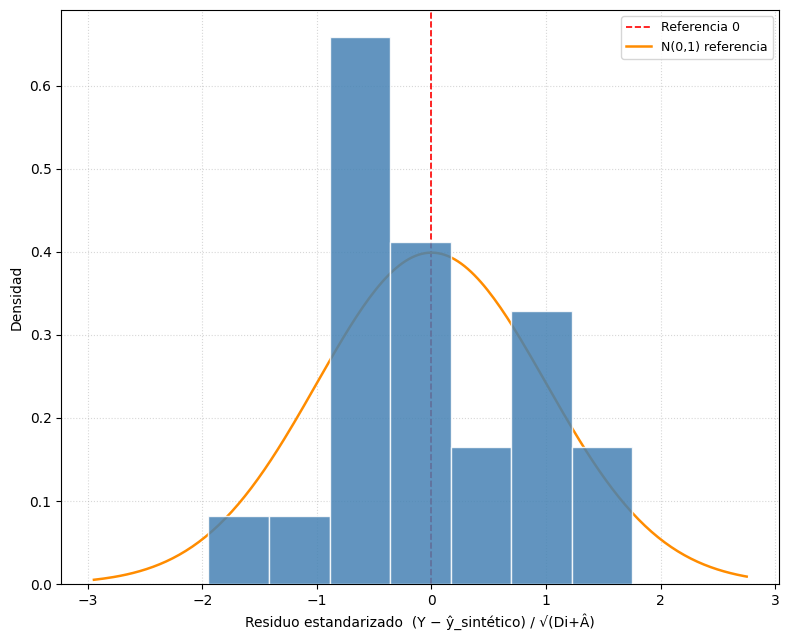
\includegraphics[width=0.48\textwidth]{img/fh_var1_histograma.png}
    \hfill
    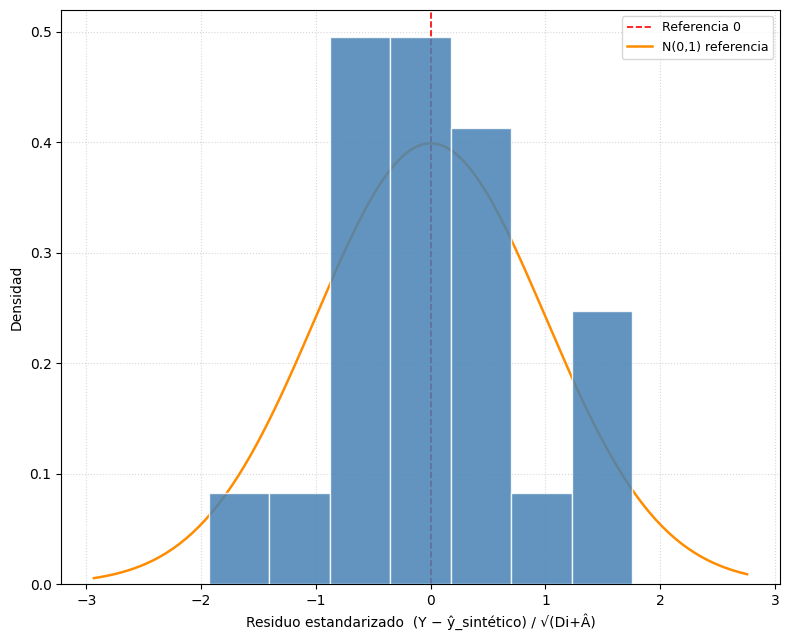
\includegraphics[width=0.48\textwidth]{img/fh_var3_histograma.png}
    \\[6pt]
    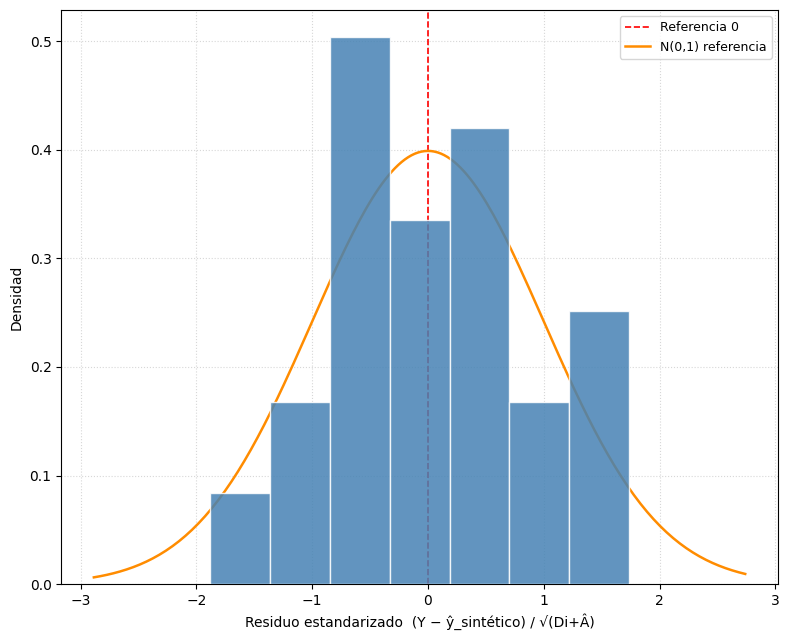
\includegraphics[width=0.48\textwidth]{img/fh_var4_histograma.png}
    \hfill
    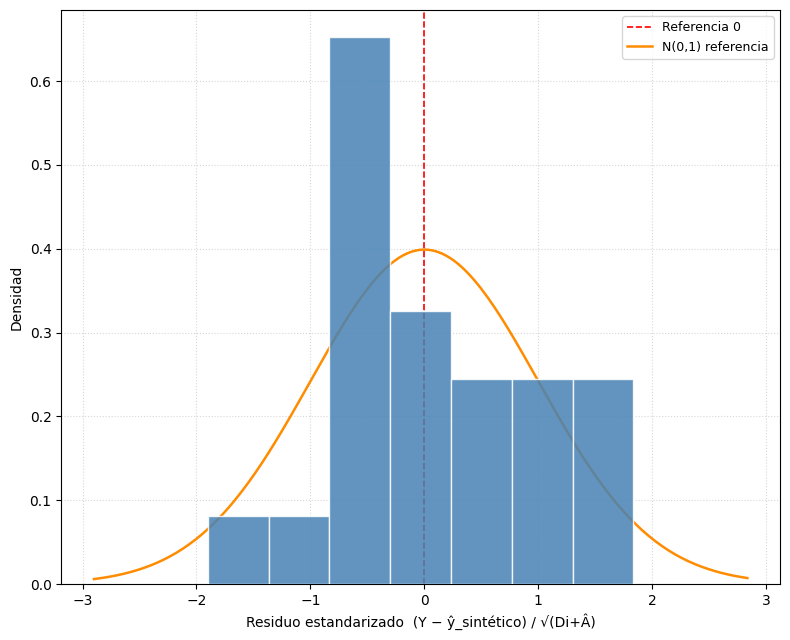
\includegraphics[width=0.48\textwidth]{img/fh_var5_histograma.png}
    \caption{Histograma de los residuos estandarizados de la Ecuación~\ref{eq:residuos} de las
             variantes no elegidas, con la misma disposición de la
             Figura~\ref{fig:ap_suavizador_variantes}: M1, M3, M4 y M5. La curva naranja es la
             densidad normal estándar de referencia y la línea roja punteada marca el cero.}
    \label{fig:ap_histograma_variantes}
    \end{figure}
    \FloatBarrier


%--------------------------------------------------------------------------------------
\section{Catálogo conceptual de covariables}
\label{sec:apendice-catalogo}

    La Tabla~\ref{tab:catalogo_literatura} reúne las veinticuatro entradas del catálogo conceptual de la Sección~\ref{subsec:met_elegibilidad}, con su código de indicador en TerriData, el signo esperado de su asociación con la tasa de desempleo y la referencia que sustenta su mecanismo. Las diecinueve primeras son las candidatas activas; las cinco últimas carecen de dato utilizable y su motivo se registra en la Tabla~\ref{tab:trazabilidad_covariables}.

    {\footnotesize
    \renewcommand{\arraystretch}{1.2}
    \setlength{\tabcolsep}{4pt}
    \begin{longtable}{>{\raggedright\arraybackslash}p{3.7cm} l
                      >{\raggedright\arraybackslash}p{3.9cm} c
                      >{\raggedright\arraybackslash}p{4.3cm}}
    \caption{Catálogo conceptual de covariables. Signo: $+$ la covariable se asocia con mayor
             desempleo, $-$ con menor desempleo y $\pm$ la literatura no fija una dirección
             única; las entradas sin dato utilizable no tienen signo asignado.}
    \label{tab:catalogo_literatura} \\
    \toprule
    \textbf{Covariable} & \textbf{Código} & \textbf{Indicador de TerriData} & \textbf{Signo} &
    \textbf{Referencia} \\
    \midrule
    \endfirsthead
    \toprule
    \textbf{Covariable} & \textbf{Código} & \textbf{Indicador de TerriData} & \textbf{Signo} &
    \textbf{Referencia} \\
    \midrule
    \endhead
    \bottomrule
    \endfoot
    \multicolumn{5}{l}{\textit{Educación}} \\
    COB\_NET\_MEDIA & 040010010 & Cobertura neta en educación media & $-$ &
        Castillo-Robayo y García-Estévez (2019), \textit{Revista Finanzas y Política Económica}, 11(1) \\
    COB\_NET\_SEC & 040010009 & Cobertura neta en educación secundaria & $-$ &
        Castillo-Robayo y García-Estévez (2019) \\
    SABER11\_MAT & 040040001 & Puntaje promedio Pruebas Saber 11, Matemáticas & $-$ &
        Castillo-Robayo y García-Estévez (2019) \\
    SABER11\_LEC & 040040002 & Puntaje promedio Pruebas Saber 11, Lectura crítica & $-$ &
        Castillo-Robayo y García-Estévez (2019) \\
    TASA\_TRAN\_EDU\_SUP & 040010028 & Tasa de tránsito inmediato a la educación superior & $-$ &
        Castillo-Robayo y García-Estévez (2019), mecanismo de capital humano \\
    \addlinespace
    \multicolumn{5}{l}{\textit{Economía}} \\
    VA\_PC & 120210002 & Valor agregado per cápita & $-$ &
        Ramírez et al. (2021), determinantes del desempleo y del empleo vulnerable \\
    VA\_PCT\_PRIM & 120210008 & Porcentaje del valor agregado, actividades primarias & $\pm$ &
        Banco de la República (2016), Reportes del Emisor 211; Bonet (2005), DTSERU 62 \\
    VA\_PCT\_SEC & 120210009 & Porcentaje del valor agregado, actividades secundarias & $\pm$ &
        Banco de la República (2016); Bonet (2005) \\
    VA\_PCT\_TERC & 120210010 & Porcentaje del valor agregado, actividades terciarias & $\pm$ &
        Banco de la República (2016); Bonet (2005) \\
    \addlinespace
    \multicolumn{5}{l}{\textit{Pobreza}} \\
    IND\_POB\_MULT & 140010004 & Índice de pobreza multidimensional (IPM) & $+$ &
        DANE (2018), medida de pobreza multidimensional municipal de fuente censal \\
    \addlinespace
    \multicolumn{5}{l}{\textit{Demografía y población}} \\
    PCT\_URBANA & 020040003 & Porcentaje de población urbana & $+$ &
        DANE, Atlas estadístico, tomo II \\
    DENS\_POB & 010010010 & Densidad poblacional & $\pm$ &
        DNP, orientaciones para la medición del desempeño de las entidades territoriales \\
    PCT\_JOVENES & 020090021 & Porcentaje de población entre 14 y 28 años & $+$ &
        Tamayo (2008), Borradores de Economía 491 \\
    \addlinespace
    \multicolumn{5}{l}{\textit{Finanzas públicas}} \\
    IDF & 070100007 & Indicador de desempeño fiscal & $-$ &
        DNP (2023), índice de desempeño fiscal municipal \\
    ING\_TRIB\_PC & 070010020 & Ingresos tributarios per cápita & $-$ &
        Fundación Felipe González (2020), empleo público de emergencia \\
    \addlinespace
    \multicolumn{5}{l}{\textit{Conflicto armado y seguridad ciudadana}} \\
    IICA\_CONFLICTO & 260020003 & Índice de Incidencia del Conflicto Armado & $+$ &
        Ibáñez (2008), desplazamiento forzoso; sustituye a las víctimas de desplazamiento \\
    TASA\_HOMICIDIOS & 060010003 & Tasa de homicidios por 100,000 habitantes & $+$ &
        \textit{Revista Panamericana de Salud Pública} (2024), determinantes sociales en Cali \\
    \addlinespace
    \multicolumn{5}{l}{\textit{Vivienda y acceso a servicios públicos}} \\
    COB\_ACUEDUCTO & 030010004 & Cobertura de acueducto (Censo) & $-$ &
        DNP (2019), Cartilla 1 de TerriData \\
    BANDA\_ANCHA & 030010003 & Penetración de banda ancha & $-$ &
        DNP (2019), Cartilla 1 de TerriData \\
    \addlinespace
    \multicolumn{5}{l}{\textit{Entradas sin dato utilizable}} \\
    TASA\_ANALFABETISMO & 040030003 & Tasa de analfabetismo (Censo) & --- & --- \\
    DENS\_EMPRESARIAL & 160080001 & Empresas generadoras de empleo formal por 10,000 habitantes & --- & --- \\
    POBREZA\_MONETARIA & 140060001 & Incidencia de la pobreza monetaria & --- & --- \\
    GINI & 140010003 & Coeficiente de Gini & --- & --- \\
    VICTIMAS\_DESPLAZAMIENTO & 260030002 & Víctimas de desplazamiento forzado ubicadas & --- & --- \\
    \end{longtable}
    }

%--------------------------------------------------------------------------------------
\section{Material complementario de Resultados}
\label{app:resultados}

Esta sección reúne tablas de apoyo de la Sección~\ref{sec:resultados} que no responden por sí solas a un objetivo; cada una se cita desde la sección de Resultados que complementa.

\subsection{Tratamiento de faltantes y atípicos}

Complementa la Sección~\ref{sec:res_faltantes}.

\begin{table}[!htbp]
\centering
\small
\caption{Resultado del tratamiento de faltantes y atípicos.}
\label{tab:res_faltantes}
\begin{tabularx}{\linewidth}{>{\raggedright\arraybackslash}p{4.6cm} >{\raggedright\arraybackslash}X}
\toprule
Caso & Resultado \\
\midrule
Factor de expansión faltante & 0 personas; el procesamiento no se detuvo \\
Registros sin código de área & \num{152314} personas de 2018 (762,753 menos 610,439 con área) no se usan; 9 capitales no tienen registros con código de área en 2018 \\
Indicadores de TerriData con faltantes en los dominios & \num{1073} de \num{1582}; salen en el pre-filtrado \\
Candidatas con faltantes en los municipios objetivo & 0 de 18 \\
Valores atípicos en las candidatas (regla del diagrama de caja) & 22 casos en 13 de las 18; Quibdó y Riohacha son los dominios que más se repiten; ninguno se eliminó \\
Valores atípicos en la tasa directa & Ninguno \\
\bottomrule
\end{tabularx}
\end{table}

\subsection{Variables de la literatura sin dato utilizable}

Complementa la Sección~\ref{sec:res_covariables}.

\begin{table}[!htbp]
\centering
\small
\caption{Variables de la revisión de literatura sin dato utilizable.}
\label{tab:res_excluidas}
\begin{tabularx}{\linewidth}{>{\raggedright\arraybackslash}p{5.2cm} >{\raggedright\arraybackslash}X}
\toprule
Variable & Motivo \\
\midrule
Tasa de analfabetismo (censo) & Sin dato en los dominios con encuesta para 2018 \\
Empresas generadoras de empleo formal por cada 10,000 habitantes & La serie termina en 2016 \\
Incidencia de la pobreza monetaria & Solo departamentos y 23 ciudades; no existe en los municipios objetivo \\
Coeficiente de Gini & Solo departamental \\
Víctimas de desplazamiento forzado ubicadas & Solo 2022 y 2023 \\
Índice de incidencia del conflicto armado & Retirado: mide el conflicto en el propio municipio; $r = 0.92$ con la tasa de homicidios en los dominios; 13 valores distintos \\
\bottomrule
\end{tabularx}
\end{table}

\subsection{Sensibilidad de las covariables de las áreas metropolitanas a la regla de agregación}

Complementa la Sección~\ref{sec:res_covariables}.

\begin{table}[!htbp]
\centering
\small
\caption{Cambio relativo máximo en los 7 dominios con A.M. entre la agregación con el denominador propio y la agregación con la población de 15 años y más. Solo se muestran las variables con cambio de 1~\% o más; en las otras 14 es menor.}
\label{tab:res_agregacion_am}
\begin{tabular}{l l r l}
\toprule
Covariable & Denominador propio & Cambio máximo (\%) & Dominio \\
\midrule
Densidad de población & Superficie & 67.67 & Bucaramanga A.M. \\
Valor agregado de actividades secundarias & Valor agregado & 43.94 & Cali A.M. \\
Valor agregado de actividades primarias & Valor agregado & 14.23 & Manizales A.M. \\
Valor agregado de actividades terciarias & Valor agregado & 8.04 & Cali A.M. \\
\bottomrule
\end{tabular}
\end{table}

\subsection{Frecuencia de selección en la validación con el procedimiento completo}

Complementa la Sección~\ref{sec:res_validacion}.

\begin{table}[!htbp]
\centering
\small
\caption{Frecuencia con que cada covariable entra en las 23 iteraciones del procedimiento completo, en la selección de covariables y en el benchmark.}
\label{tab:res_frecuencia}
\begin{tabular}{l r r}
\toprule
Covariable & Selección (\%) & Benchmark (\%) \\
\midrule
Tasa de homicidios & 78.26 & 69.57 \\
Cobertura de acueducto & 56.52 & 8.70 \\
Cobertura neta en educación media & 8.70 & 4.35 \\
Ingresos tributarios per cápita & 4.35 & 4.35 \\
Valor agregado de actividades primarias & 4.35 & 4.35 \\
Ninguna (solo intercepto) & 17.39 & 17.39 \\
\bottomrule
\end{tabular}
\end{table}

\subsection{Validación dejar-un-dominio-fuera del modelo espacial}

Complementa la Sección~\ref{sec:res_espacial}.

\begin{table}[!htbp]
\centering
\small
\caption{Validación predictiva dejar-un-dominio-fuera con la tasa de homicidios fija, escenario de referencia (3 vecinos, estructura completa). Errores en puntos porcentuales. Las métricas de los cuatro escenarios están en el Apéndice~\ref{app:espacial}.}
\label{tab:res_validacion_espacial}
\begin{tabular}{l r r r r r}
\toprule
Estimador del dominio retirado & RMSE & MAE & Sesgo & Cobertura (\%) & Habilidad \\
\midrule
Sintético clásico & 2.52 & 2.13 & $-0.07$ & 100.00 & 0.17 \\
Sintético espacial & 2.48 & 2.09 & $-0.07$ & 100.00 & 0.20 \\
Espacial con efecto & 2.35 & 1.99 & $-0.03$ & 100.00 & 0.28 \\
Solo intercepto & 2.77 & 2.23 & $-0.01$ & 95.65 & no aplica \\
\bottomrule
\end{tabular}
\end{table}

\FloatBarrier

%--------------------------------------------------------------------------------------
\section{Repositorio de github}
\label{sec:repositorio-github}

https://github.com/juanp001/Estimacion-desempleo-Colombia-SAE

